% !TEX root = main.tex

\subsection{基本概念}
\subsubsection{单周期CPU}
\qquad单周期CPU是指CPU的每条指令都在一个时钟周期内完成,通常在每个时钟周期的上升沿触发。
\par CPU在处理指令时一般要经过以下五个阶段:
\begin{enumerate}
	\item 取指(IF):根据程序计数器PC中的指令地址,从存储器中取出一条指令,同时,PC根据指令字长度自动递增产生下一条指令所需要的指令地址;但遇到``地址转移''指令时,则需要对``转移地址''进行处理后送入PC。
	\item 译码(ID):对取指操作中得到的指令进行译码,确定该指令需要完成的操作,从而产生相应的操作控制信号,用于下一步的执行。
	\item 执行(EXE):根据指令译码得到的操作控制信号,执行指令动作。
	\item 访存(MEM):所有需要访问存储器的操作都将在这个步骤中执行,该步骤给出存储器的数据地址,把数据写入到存储器中数据地址所指定的存储单,或者从存储器中得到数据地址单元中的数据。
	\item 写回(WB):将指令执行的结果或者访问存储器得到的数据写回相应的目标寄存器。
\end{enumerate}

\subsubsection{数据通路及控制信号}
\qquad 基本数据通路见图\ref{fig:datapath},控制信号见表\ref{tab:control}。
\begin{figure}[H]
\centering
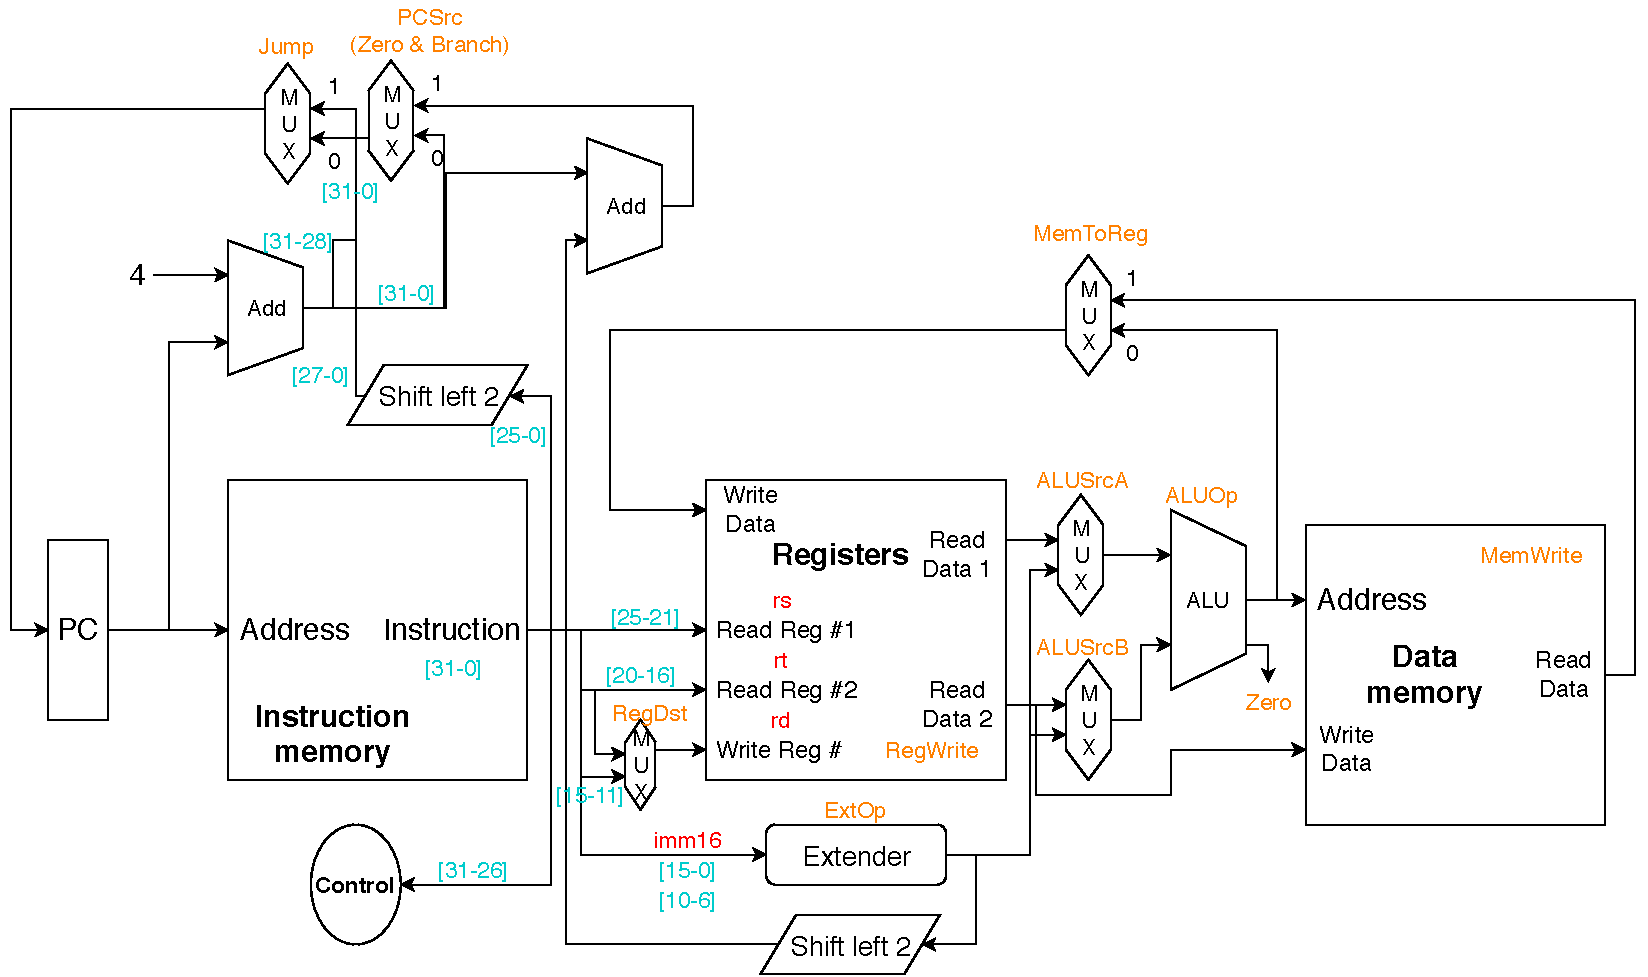
\includegraphics[width=\linewidth]{fig/Datapath.pdf}
\caption{基本数据通路}
\label{fig:datapath}
\end{figure}
\begin{table}[H]
  \centering\xiaowu
  \caption{控制信号}
    \begin{tabular}{|l|l|l|}
    \hline
    \multicolumn{1}{|c|}{控制信号名} & \multicolumn{1}{c|}{状态0} & \multicolumn{1}{c|}{状态1} \bigstrut\\
    \hline
    Reset & 初始化PC为0 & PC接收新地址 \bigstrut\\
    \hline
    PCWre & PC不更改,halt & PC更改 \bigstrut\\
    \hline
    RegDst & 写入寄存器地址来自rt字段 & 写入寄存器地址来自rd字段 \bigstrut\\
    \hline
    RegWrite & 寄存器不可写 & 寄存器可写 \bigstrut\\
    \hline
    ALUSrcA & 寄存器rs内容 & 立即数sa \bigstrut\\
    \hline
    ALUSrcB & 寄存器rt内容 & 立即数imm \bigstrut\\
    \hline
    ExtOp & 零扩展   & 符号扩展 \bigstrut\\
    \hline
    ALUOp & \multicolumn{2}{c|}{见表\ref{tab:alu_op}} \bigstrut\\
    \hline
    MemToReg & ALU输出 & 内存读取 \bigstrut\\
    \hline
    MemWrite & 内存不可写 & 内存可写 \bigstrut\\
    \hline
    Branch & 非分支   & 分支 \bigstrut\\
    \hline
    Jump  & 非跳转   & 跳转 \bigstrut\\
    \hline
    \end{tabular}%
  \label{tab:control}%
\end{table}%

\subsubsection{MIPS指令格式}
\qquad MIPS指令可分为以下三种格式,见图\ref{fig:mips_type}。
\begin{figure}[htbp]
\centering
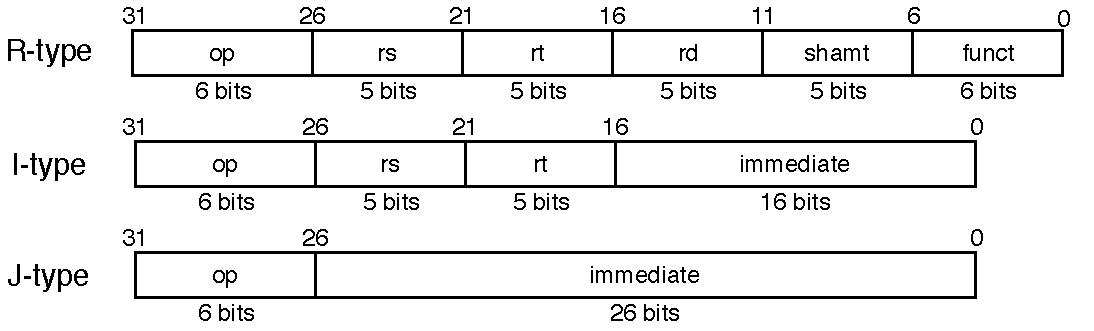
\includegraphics[width=0.8\linewidth]{fig/MIPS.pdf}
\caption{MIPS指令类型}
\label{fig:mips_type}
\end{figure}
其中各字段缩写含义如表\ref{tab:mips}所示。
% Table generated by Excel2LaTeX from sheet 'Sheet1'
\begin{table}[htbp]
  \centering\xiaowu
  \caption{\xiaowu MIPS指令各字段缩写含义}
    \begin{tabular}{|l|l|}
    \hline
    op    & 操作码 \bigstrut\\
    \hline
    rs    & 只读,第一个源操作数寄存器地址/编号,范围为\verb'0x00'$\sim$\verb'0x1F' \bigstrut\\
    \hline
    rt    & 可读可写,第二个源操作数地址或目标操作数寄存器地址 \bigstrut\\
    \hline
    rd    & 只写,目的操作数寄存器地址 \bigstrut\\
    \hline
    sham(shift amt) & 位移量,在移位指令中用于指定移多少位 \bigstrut\\
    \hline
    funct & 功能码,在R类型指令中配合op一起使用 \bigstrut\\
    \hline
    immediate & 16位立即数 \bigstrut\\
    \hline
    address & 目标转移地址 \bigstrut\\
    \hline
    \end{tabular}%
  \label{tab:mips}%
\end{table}%